\documentclass[handout]{beamer}
\usepackage{verbatim}
\usepackage{xcolor}
\usepackage{multirow}
\usepackage{amssymb}
\usepackage{tikz}
\usepackage{hyperref}
\usetikzlibrary{positioning,fit}
%\usepackage{enumitem}
\usetheme{Warsaw}
\setbeamertemplate{navigation symbols}{}
\newcommand{\blue}[1]{{\color{blue} #1}}
\newcommand{\red}[1]{{\color{red} #1}}
\newcommand{\grn}[1]{{\color{green} #1}}
\newcommand{\bluRed}[2]{{\color{blue} #1}{\color{red} #2}}
\newcommand{\qtns}[0]{\begin{center} Questions? \end{center}}
\newcommand{\nl}[1]{\vspace{#1 em}}
\newcommand{\cntrImg}[2]{\begin{center}\includegraphics[scale=#2]{#1}\end{center}}
\newcommand{\defn}[1]{{\bf #1}}
\let\emptyset\varnothing
\newcommand{\SampS}[0]{$\mathcal{S}$}

\title{Math 3070, Applied Statistics}

\begin{document}
\begin{frame}
    \begin{beamercolorbox}[rounded=true,wd=\textwidth,center]{title}
        \usebeamerfont{title}\inserttitle
    \end{beamercolorbox}
    \begin{center}
        Section 1\\
        \nl{0.5}
        September 30, 2019
    \end{center}
\end{frame}
\begin{frame}{Lecture Outline, 9/30}
    Section 4.5 and 4.6
    \begin{itemize}
        \item Gamma Function
        \item Weibull Distribution
        \item Lognormal Distribution
        \item Beta Distribution
        \item Probability Plots
    \end{itemize}
\end{frame}
\begin{frame}{Gamma Function, Summary}
    \begin{block}{}
        \begin{itemize}
            \item $\Gamma(k) = \int_{0}^\infty x^{k-1}e^{-x} dx$
            \item $ \Gamma(1) = 1 $
            \item $ \Gamma(1/2) = \sqrt{\pi} $
            \item $ \Gamma(k+1) = k\Gamma(k), \hskip1 em k>0$
            \item $ \Gamma(k+1) = k!, \hskip1 em \text{integer } k$
        \end{itemize}
    \end{block}
    \begin{align*}
        \Gamma(k+1) & = \int_{0}^\infty x^{k}e^{-x} dx                                    \\
                    & = -x^{k}e^{-x}\bigg|_{x=0}^\infty + k\int_0^\infty x^{k-1}e^{-x} dx \\
                    & = 0+ k\Gamma(k)                                                     \\
    \end{align*}
    \vfill
\end{frame}
\begin{frame}{Weibull Distribution, PDF}
    \begin{block}{}
        A \textbf{Weibull} random variable $X$ with shape $\alpha>0$ and scale $\beta>0$ has pdf
        $$f(x)=\begin{cases}\frac{\alpha}{\beta^\alpha}x^{\alpha-1}e^{-(x/\beta)^\alpha}, & x\geq 0 \\ 0, & x<0\end{cases}$$
        $X\sim Weibull(\alpha, \beta)$
    \end{block}
    \begin{center}
        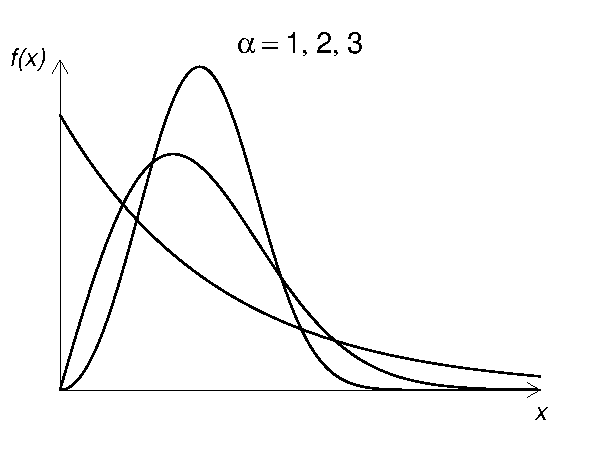
\includegraphics[scale=.4]{ch4_pdf_weibull.pdf}
    \end{center}
    Important for central limit theorems involving extreme values. For example, $\max(X_1, X_2,\ldots X_n)$ or $\min(X_1, X_2,\ldots X_n)$ as $n\to \infty$.
\end{frame}
\begin{frame}{Weibull Distribution, Check PDF}
    Suppose $X\sim Weibull(\alpha, \beta)$.\\
    \uncover<1->{$f(x)\geq 0$.}
    \begin{align*}
        \uncover<2->{\int_{-\infty}^\infty f(x)dx & =} \uncover<3->{\int_{0}^\infty \frac{\alpha}{\beta^\alpha}x^{\alpha-1}e^{-(x/\beta)^\alpha}dx}                            \\
        \uncover<4->{\text{use } u = x^\alpha     & \to du = \alpha x^{\alpha-1} dx }                                                                                          \\
                                                  & \uncover<5->{= \int_{0}^\infty \frac{e^{-x^\alpha/\beta^\alpha}}{\beta^\alpha} \alpha x^{\alpha-1}dx} \\
                                                  & \uncover<6->{= \int_{0}^\infty \frac{e^{-u/\beta^\alpha}}{\beta^\alpha} du}                                                \\
                                                  & \uncover<7->{= -e^{-u/\beta^\alpha}\bigg|_{u=0}^\infty = -e^{-(x/\beta)^\alpha}\bigg|_{x=0}^\infty }                       \\
                                                  & \uncover<8->{= 0 - (-1) = 1}                                                                                               \\
    \end{align*}
    \uncover<8->{$f(x)$ is a PDF.}
    \vfill
\end{frame}
\begin{frame}{Weibull Distribution, CDF}
    Suppose $X\sim Weibull(\alpha, \beta)$. The previous calculation shows us how to calculate the CDF.
    \begin{align*}
        \uncover<1->{F(x) = P(X<x) = \int_{-\infty}^x f(y)dy & = \int_{0}^x \frac{\alpha}{\beta^\alpha}y^{\alpha-1}e^{-(y/\beta)^\alpha}dy} \\
        \uncover<2->{                                        & = -e^{-(y/\beta)^\alpha}\bigg|_{y=0}^x }                                     \\
        \uncover<3->{                                        & = -e^{-(x/\beta)^\alpha}-(-1) }                                              \\
        \uncover<3->{                                        & = 1-e^{-(x/\beta)^\alpha}}                                                   \\
    \end{align*}
    \vfill
\end{frame}
\begin{frame}{Weibull Distribution, Expected Value}
    Suppose $X\sim Weibull(\alpha, \beta)$.\\
    \begin{align*}
        E[X] = \uncover<1->{\int_{-\infty}^\infty x f(x)dx} & = \uncover<2->{\int_{0}^\infty x \frac{\alpha}{\beta^\alpha}x^{\alpha-1}e^{-(x/\beta)^\alpha}dx} \\
        \uncover<3->{\text{use } u = (x/\beta)^\alpha       & \to du = \alpha \frac{x^{\alpha-1}}{\beta^\alpha} dx  \text{ and } x = \beta u^{1/\alpha}}       \\
                                                            & \uncover<4->{= \int_{0}^\infty x e^{-u}  du = \beta \int_{0}^\infty u^{1/\alpha} e^{-u}du}       \\
                                                            & \uncover<5->{= \beta \int_{0}^\infty u^{(1 + 1/\alpha)-1} e^{-u}du}                              \\
                                                            & \uncover<6->{= \beta \Gamma \bigg( 1 + \frac{1}{\alpha} \bigg)}                                  \\
    \end{align*}
    \vfill
\end{frame}
\begin{frame}{Weibull Distribution, Variance}
    Suppose $X\sim Weibull(\alpha, \beta)$.\\
    Use $Var(X) = E[X^2] - E[X]^2$
    \begin{align*}
        \uncover<1->{ E[X^2] = \int_{-\infty}^\infty x^2 f(x)dx} & = \uncover<2->{\int_{0}^\infty x^2 \frac{\alpha}{\beta^\alpha}x^{\alpha-1}e^{-(x/\beta)^\alpha}dx}                                        \\
        \uncover<3->{\text{use } u = (x/\beta)^\alpha            & \to du = \alpha \frac{x^{\alpha-1}}{\beta^\alpha} dx  \text{ and } x = \beta u^{1/\alpha}}                                                \\
                                                                 & \uncover<4->{= \int_{0}^\infty x^2 e^{-u}  du = \beta^2 \int_{0}^\infty u^{2/\alpha} e^{-u}du}                                            \\
                                                                 & \uncover<5->{= \beta^2 \int_{0}^\infty u^{(1 + 2/\alpha)-1} e^{-u}du}                                                                     \\
                                                                 & \uncover<6->{= \beta^2 \Gamma \bigg( 1 + \frac{2}{\alpha} \bigg)}                                                                         \\
        \uncover<7->{V(X) = E[X^2] - E[X]^2                      & = \beta^2 \bigg[ \Gamma \bigg( 1 + \frac{2}{\alpha} \bigg) - \Gamma \bigg( 1 + \frac{1}{\alpha} \bigg)^2 \bigg] \\}
    \end{align*}
\end{frame}
\begin{frame}{Weibull Distribution, Expected Value Example}
    Suppose that $X \sim Weibull(2,\beta)$ and $E[X] = 3$. Determine $\beta$, the scale parameter.
    \begin{align*}
        \uncover<1->{3 = E[X]  & = \beta \Gamma\bigg(1 + \frac{1}{2}\bigg) }        \\
        \uncover<2->{          & = \beta \frac{1}{2}\Gamma\bigg(\frac{1}{2}\bigg) } \\
        \uncover<3->{          & = \beta \frac{1}{2}\sqrt{\pi} }                    \\
        \uncover<4->{\to \beta & = \frac{6}{\sqrt{\pi}} }                           \\
    \end{align*}
    \vfill
\end{frame}
\begin{frame}{Weibull Distribution, Typical Example}
    Suppose that $X \sim Weibull(2,3)$. What is the probability that $X$ is greater than $3$.
    \begin{align*}
        \uncover<1->{P(X>3)} \uncover<2->{ & = 1 - P(X\leq 3) }                  \\
        \uncover<3->{                      & \text{use the CDF} }                \\
        \uncover<4->{                      & = 1 - (1 - e^{-(3/\beta)^\alpha}) } \\
        \uncover<5->{                      & = e^{-(3/3)^2} = e^{-1}}            \\
    \end{align*}
    \vfill
\end{frame}
\begin{frame}{Weibull Distribution, Summary}
    \begin{itemize}
        \item $X\sim Weibull(\alpha, \beta)$
        \item $$f(x)=\begin{cases}\frac{\alpha}{\beta^\alpha}x^{\alpha-1}e^{-(x/\beta)^\alpha}, & x\geq 0 \\ 0, & x<0\end{cases}$$
        \item $$F(x)=\begin{cases}1 -e^{-(x/\beta)^\alpha} , & x\geq 0 \\ 0, & x<0\end{cases}$$
        \item $$ E[X] = \beta\Gamma\bigg( 1 + \frac{1}{\alpha} \bigg) \hskip 2em V(X) = \beta^2\bigg[\Gamma\bigg( 1 + \frac{2}{\alpha} \bigg) - \bigg( 1 + \frac{1}{\alpha} \bigg)^2\bigg] $$
        \item Think of this if you need a central limit theorem for extreme values later in life.\\
              \url{https://en.wikipedia.org/wiki/Extreme_value_theory}
    \end{itemize}
\end{frame}
\begin{frame}{Log-normal Distribution, Introduction}
    \begin{block}{}
        A random variable $X$ is said to have a \textbf{log-normal} distribution if $\ln(X)$ is a normal random variable $N(\mu,\sigma)$.\\
        $X\sim Lognormal(\mu, \sigma)$
    \end{block}

    A log-normal random variable $X$ may be written in the form $X=e^{\sigma  Z+\mu}$, where $Z$ is a standard normal random variable.
    \begin{center}
        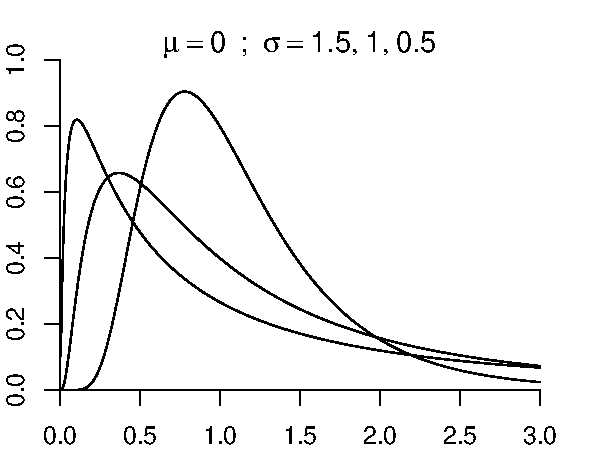
\includegraphics[scale=0.5]{ch4_pdf_logn.pdf}
    \end{center}
    Used with Black-Scholes and other compound rate models. \\
    Note, $\propto$ should be $\mu$ in the plot.
\end{frame}
\begin{frame}{Log-normal Distribution, CDF}
    Suppose $X\sim Lognormal(\mu,\sigma)$.
    \begin{align*}
        \uncover<1->{ F(x) & = P(X< x)}                              \uncover<2->{ = P(e^{\sigma Z + \mu}<x) }                      \\
                                                                      & \uncover<3->{ = P\bigg( Z<\frac{\ln(x) - \mu}{\sigma} \bigg) } \\
                                                                      & \uncover<4->{ = \Phi\bigg(\frac{\ln(x) - \mu}{\sigma} \bigg) } \\
        \uncover<5->{\text{range of log all real numbers and }        & \text{domain is } (0,\infty) }                                 \\
        \uncover<6->{( 0, \infty] \text{ are the possible values of } & X  }                                                           \\
    \end{align*}
    \uncover<7->{$$F(x) =\begin{cases} \Phi\bigg(\frac{\ln(x) - \mu}{\sigma} \bigg), & x> 0 \\ 0, & x\leq 0\end{cases} $$ }
\end{frame}
\begin{frame}{Log-normal Distribution, PDF}
    Suppose $X\sim Lognormal(\mu,\sigma)$.\\
    \uncover<1->{Differentiate for PDF.}\\
    \uncover<2->{$f(x) = 0$ when $x\leq 0 \to F(x) =0$ when $x\leq 0$}
    \uncover<3->{When $x>0$,}
    \begin{align*}
        \uncover<3->{\frac{d}{dx} \Phi\bigg(\frac{\ln(x) - \mu}{\sigma} \bigg)  } & \uncover<4->{ = \Phi'\bigg(\frac{\ln(x) - \mu}{\sigma} \bigg) \bigg[ \frac{d}{dx} \frac{\ln(x) - \mu}{\sigma} \bigg] } \\
                                                                                  & \uncover<5->{ = \frac{1}{\sigma x} \Phi'\bigg(\frac{\ln(x) - \mu}{\sigma} \bigg)  }                                    \\
                                                                                  & \uncover<6->{ = \frac{1}{\sigma x} \frac{1}{\sqrt{2\pi}} \exp\bigg( \frac{-[\ln(x) - \mu]^2}{2 \sigma^2}\bigg)  }      \\
    \end{align*}
    \uncover<7->{Is a PDF since the CDF was known.}
    \uncover<8->{$$f(x) =\begin{cases} \frac{1}{\sqrt{2\pi}\sigma x} \exp\bigg( \frac{-[\ln(x) - \mu]^2}{2 \sigma^2}\bigg), & x> 0 \\ 0, & x\leq 0\end{cases} $$ }
    \vfill
\end{frame}
\begin{frame}{Log-normal Distribution, Mean}
    Suppose $X\sim Lognormal(\mu,\sigma)$.\\
    \vspace{-1em}
    \begin{align*}
        \uncover <1-> {E[X]              & = \int_{-\infty}^\infty x f(x) dx =}  \uncover<2->{\int_{0}^\infty \frac{x}{\sqrt{2\pi}} \exp\bigg( \frac{-[\ln(x) - \mu]^2}{2 \sigma^2}\bigg) \frac{dx}{\sigma x}}                       \\
        \uncover<3->{ \text{use u-sub: } & y = \frac{\ln(x) -\mu}{\sigma} \to x = e^{\sigma y + \mu}, \hskip 0.3em dy = \frac{dx}{\sigma x}}                                                                                         \\
        \uncover<4->{                    & = \int_{-\infty}^\infty \frac{1}{\sqrt{2\pi}} \exp(\red{\sigma y + \mu}) \exp(\blue{-y^2/2}) dy }                                                                                         \\
        \uncover<5->{                    & = \int_{-\infty}^\infty \frac{1}{\sqrt{2\pi}} \exp\bigg( \blue{-\bigg[\frac{y^2}{2}} -  \red{\frac{\sigma y}{2} } +\frac{\sigma^2}{2} \bigg] + \red{\mu} + \frac{\sigma^2}{2} \bigg) dy } \\
        \uncover<6->{                    & = \int_{-\infty}^\infty \frac{1}{\sqrt{2\pi}} \exp\bigg( \frac{-(y-\sigma)^2}{2} \bigg) \exp\bigg( \mu +  \frac{\sigma^2}{2} \bigg) dy }                                                  \\
        \uncover<7->{                    & = \exp\bigg( \mu +  \frac{\sigma^2}{2} \bigg) \int_{-\infty}^\infty \frac{1}{\sqrt{2\pi}} \exp\bigg( \frac{-(y-\sigma)^2}{2} \bigg)  dy }                                                 \\
        \uncover<8->{                    & = \exp( \mu + \sigma^2/2 ), \text{ used } \int_{-\infty}^\infty f(x) dx =1 \text{ for } N(\sigma,1)}                                                                                      \\
    \end{align*}
\end{frame}
\begin{frame}{Log-normal Distribution, Variance}
    Suppose $X\sim Lognormal(\mu,\sigma)$. \\\uncover<1->{Use the same trick and $V(X) = E[X^2] - E[X]^2$}\\
    \vspace{-1.2em}
    \begin{align*}
        \uncover <1-> {E[X^2]            & = \int_{-\infty}^\infty x^2 f(x) dx =}  \uncover<2->{\int_{0}^\infty \frac{x^2}{\sqrt{2\pi}} \exp\bigg( \frac{-[\ln(x) - \mu]^2}{2 \sigma^2}\bigg) \frac{dx}{\sigma x}}                \\
        \uncover<3->{ \text{use u-sub: } & y = \frac{\ln(x) -\mu}{\sigma} \to x = e^{\sigma y + \mu}, \hskip 0.3em dy = \frac{dx}{\sigma x}}                                                                                      \\
        \uncover<4->{                    & = \int_{-\infty}^\infty \frac{1}{\sqrt{2\pi}} \exp(\red{2 \sigma y + 2 \mu}) \exp(\blue{-y^2/2}) dy }                                                                                  \\
        \uncover<5->{                    & = \int_{-\infty}^\infty \frac{1}{\sqrt{2\pi}} \exp\bigg( \blue{-\bigg[\frac{y^2}{2}} -  \red{\frac{4 \sigma y}{2} } +\frac{4 \sigma^2}{2} \bigg] +\red{2 \mu} + 2 \sigma^2 \bigg) dy } \\
        \uncover<6->{                    & = \int_{-\infty}^\infty \frac{1}{\sqrt{2\pi}} \exp\bigg( \frac{-(y-2 \sigma)^2}{2} \bigg) \exp( 2 \mu +  2 \sigma^2) dy }                                                              \\
        \uncover<7->{                    & = \exp( 2 \mu + 2 \sigma^2 ), \text{ used } \int_{-\infty}^\infty f(x) dx =1 \text{ for } N(2\sigma,1)}                                                                                \\
        \uncover<8->{ V(X)               & = e^{2\sigma^2 + 2 \mu} - e^{ \sigma^2 +  2\mu}  = e^{2\mu+\sigma^2}[e^{\sigma^2} -1]}                                                                                                 \\
    \end{align*}
\end{frame}
\begin{frame}{Log-normal Distribution, Typical Example}
    $X\sim Lognormal(1,2)$. \\Compute the probability $X$ is greater than $e^2$.
    \begin{align*}
        \uncover<1->{ P(X\geq e^2 ) & = 1 - P(X< e^2)}                                         \\
        \uncover<2->{ P(X<e^2 )     & =} \uncover<3->{P(\ln(X)< \ln[e^2]) = P(\ln(X)< 2)}      \\
        \uncover<4->{               & =P\bigg( \frac{\ln(X) -1}{2} < \frac{2-1}{2} \bigg)}     \\
        \uncover<5->{               & =P\bigg(Z < \frac{1}{2} \bigg), \hskip 1em Z\sim N(0,1)} \\
        \uncover<6->{               & =\Phi\bigg(\frac{1}{2} \bigg) \approx 0.6915}            \\
        \uncover<7->{ P(X\geq e^2 ) & \approx 1 - 0.6915 = 0.3085}                             \\
    \end{align*}
\end{frame}
\begin{frame}{Log-normal Distribution, Normal Example (Pun Intended)}
    Internet browsing time $X$ is modeled by a log normal distribution. One researcher claims that $\ln(X)$ has a mean of 5 log minutes while another claims that $X$ has an expected value of 150 minutes. Can both claims be true?\\ \nl{0.5}
    \uncover<1->{Check if these parameters are valid.}
    \begin{align*}
        \uncover<2->{5 = E[\ln(X)] &  = \mu}                             \\
        \uncover<3->{150 = E[X] & = e^{\mu + \sigma^2/2}}                            \\
        \uncover<3->{& = e^{5 + \sigma^2/2}}\\
        \uncover<4->{\ln(150) & = 5 + \sigma^2/2} \\
        \uncover<5->{\sigma^2 &= 2*(\ln(150)-5)} \\
        \uncover<6->{& \approx -0.11671515478<0} \\
    \end{align*}
    \vskip -1.5em
    \uncover<7->{Variances cannot be negative. This situation is impossible.}\\
    \uncover<8->{Moreover, the expected value of two related quantities revealed variance of one of them. Ain't that something?}
    \vfill
\end{frame}
\begin{frame}{Log-Normal, Summary}
    \begin{itemize}
        \item $X\sim Lognormal(\mu,\sigma) \iff \ln(X) \sim N(\mu, \sigma)$
        \item PDF
              $$f(x) =\begin{cases} \frac{1}{\sqrt{2\pi}\sigma x} \exp\bigg( \frac{-[\ln(x) - \mu]^2}{2 \sigma^2}\bigg), & x> 0 \\ 0, & x\leq 0\end{cases} $$
        \item CDF is not given. Related it to $\Phi$ using natural log.
        \item $$ E[X] = e^{\mu + \sigma^2/2} \hskip 2em V(X) = e^{2\mu + \sigma^2}(e^{\sigma^2} - 1) $$
    \end{itemize}
\end{frame}
\begin{frame}{Beta Distribution}     
    $X$ is a \textbf{Beta} random variable with parameters $\alpha,\beta,A$ and $B$ if it has the following PDF,
    $$f(x) =\begin{cases} \dfrac{1}{B-A}\cdot \dfrac{\Gamma(\alpha + \beta)}{\Gamma(\alpha) \cdot \Gamma(\beta)} \bigg( \dfrac{x-A}{B-A} \bigg)^{\alpha-1} \bigg( \dfrac{B-x}{B-A} \bigg)^{\beta-1} , & A\leq x \leq B \\ 0, & \text{otherwise}\end{cases} $$
        \\ \nl{0.5}
        \begin{itemize}
            \item Nonzero on a bounded interval.
            \item Sometimes appears when modeling random ratios. For example, the ratio of two gammas.
            \item Will not ask anything about it in this course. No, not even extra credit. If someone asks, we briefly discussed it. Feel free to ask me about it.
        \end{itemize}
        \vfill
\end{frame}
\begin{frame}{Probability Plots}     
Goal: assess if data follows a theoritical distribution.
\\
Idea: Plot the percentiles of the data (y-axis) versus the theoritical percentiles (x-axis) to see if they match.\\
\begin{center}
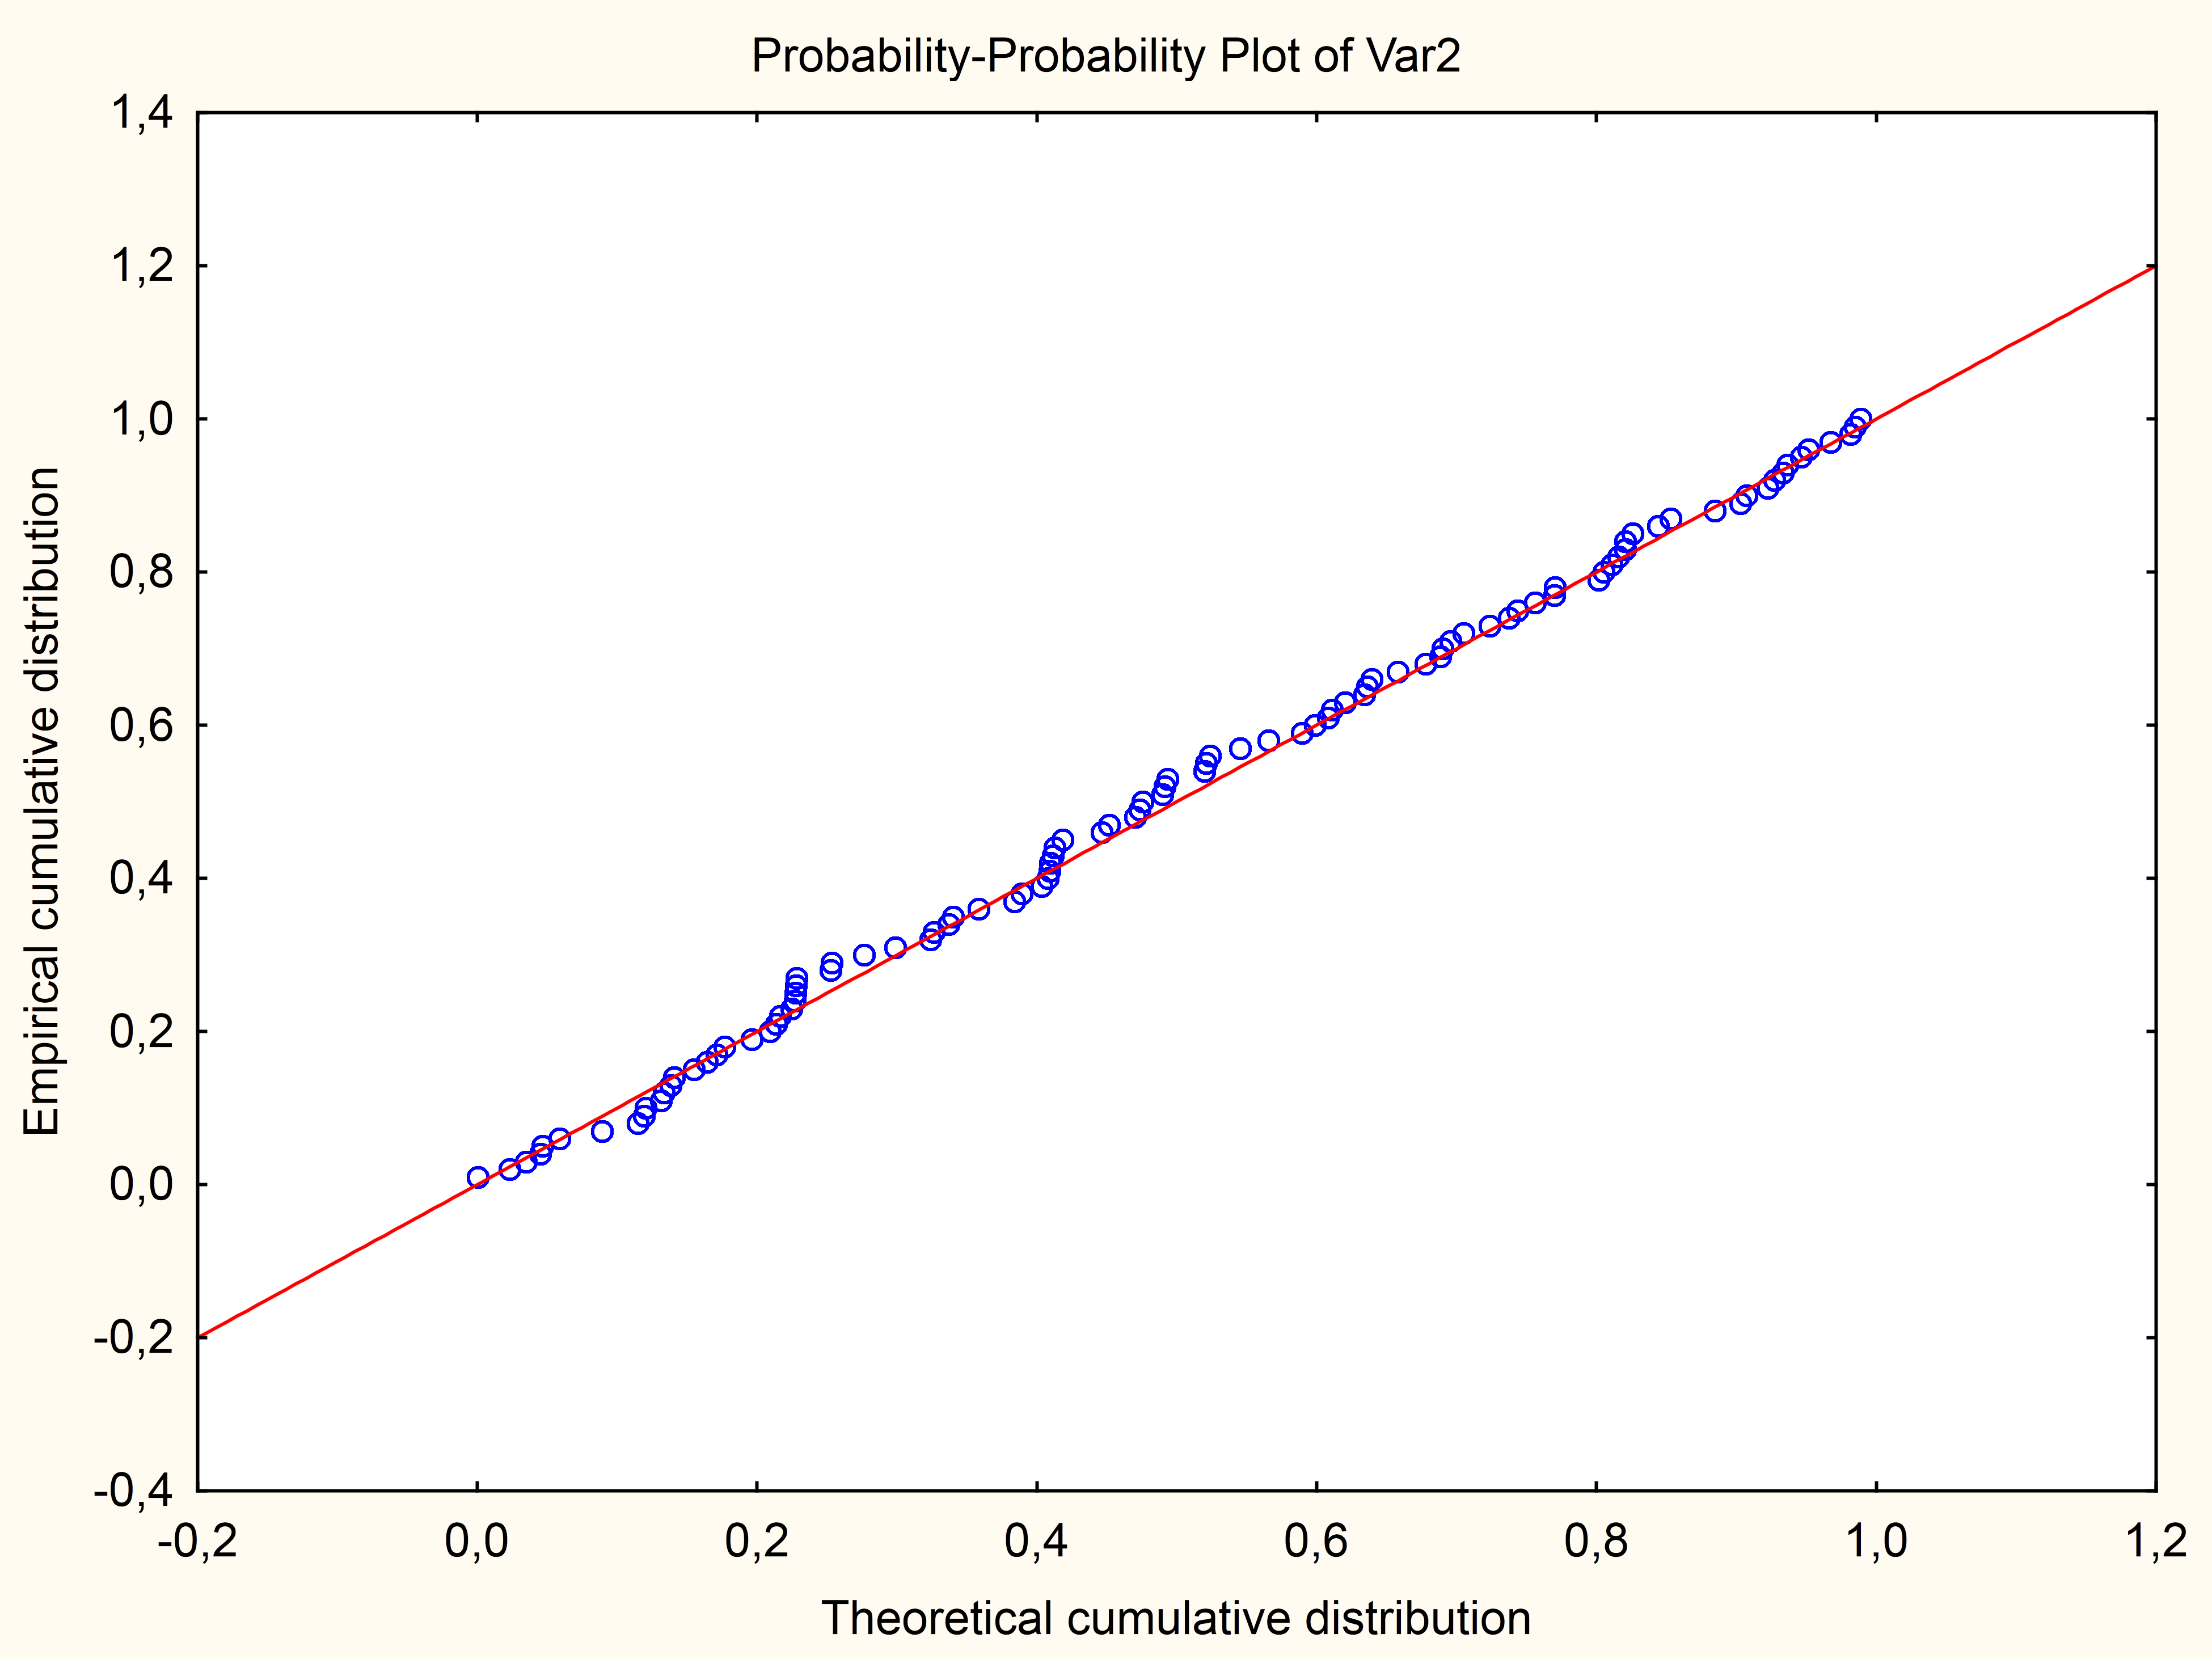
\includegraphics[scale=0.06]{PP_Plot_Wiki.png}
\end{center}
Note: Linear relationships in the plot translate to changes in mean and variance, suggesting ways to adjust parameters. Will not test over probability plots. Will appear in R Lab.
\end{frame}
\end{document}